\documentclass{article}
\usepackage{graphicx}
\usepackage[margin=1.5cm]{geometry}
\usepackage{amsmath}

\begin{document}

\title{Monday Reading Assessment: Unit 4, Sources of Magnetic Fields}
\author{Prof. Jordan C. Hanson}

\maketitle

\section{Memory Bank}

\begin{itemize}
\item $d\vec{B} = \frac{\mu_0 I}{4\pi} \frac{d\vec{l}\times\hat{r}}{r^2}$ ... Biot-Savart Law
\item $\vec{B} = (\mu_0 I) / (2 \pi r) \hat{z}$ ... B-field of a current I a distance $r$ away from the conductor carrying the current.  The direction $\hat{z}$ is given by the right-hand rule \#2 (RHR-2).
\end{itemize}

\begin{figure}[ht]
\centering
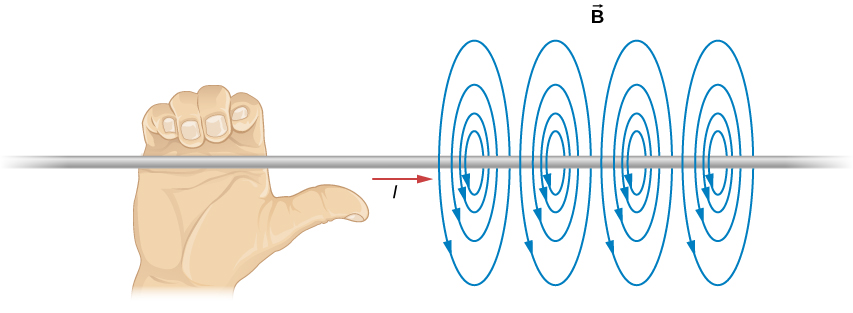
\includegraphics[width=0.75\textwidth]{wireBfield.jpeg}
\caption{\label{fig:fields} The B-field of a wire surrounding a current-carrying wire.}
\end{figure}

\section{Magnetic Forces on a Wire}

\begin{enumerate}
\item Consider Fig. \ref{fig:fields}.  (a) Define a coordinate system that describes the three directions in the problem: the vector pointing some distance away from the wire, the direction of the current, and the direction of the B-field some distance away from the wire.  All three directions should be mutually perpendicular. (b) What is the B-field vector 1 cm below the wire, if the current is 10 A? \\ \vspace{2cm}
\item Suppose a row of charges was motionless a distance $y$ \textit{above} the wire.  What would happen to the charges if the wire moved \textit{towards} them?
\end{enumerate}

\end{document}
